\documentclass[smallextended]{svjour3}

%% Language and font encodings
\usepackage[english]{babel}
\usepackage[utf8x]{inputenc}
\usepackage[T1]{fontenc}

%% Sets page size and margins
\usepackage[a4paper,top=3cm,bottom=2cm,left=3cm,right=3cm,marginparwidth=1.75cm]{geometry}

%% Useful packages
\usepackage{amsmath}
\usepackage{graphicx}
\usepackage[colorinlistoftodos]{todonotes}
\usepackage[colorlinks=true, allcolors=blue]{hyperref}
\usepackage{subcaption}
\usepackage{algorithm}
\usepackage{algorithmic}

\title{TER Report - Interior 3D detection in a cobotics context}

\author{BIZARD Astor  \\ \and \\
      Supervised by : Olivier Aycard  \and Jerôme Maisonnasse
}

\institute{
}

\date{June 2017}

\begin{document}
\maketitle

\begin{abstract}
We present an approach to compute 3D data in a real-time security context to evaluate distance between humans and robots. The implementation is oriented to be compatible with the ROS platform, and overcome drawbacks of low-quality depth cameras, such as important noise.
\keywords{3D Depth Sensor \and RGB-D Perception \and Collision Avoidance \and ROS \and Physical Human-Robot Interaction}
\end{abstract}

\section{Introduction}

The problem of collaboration between humans and industrial robots - also known as cobotics - induces security issues : how to ensure the security of the human, without limiting the possibilities of the collaboration ? We thus need to find a way to do this without preventing the humans to approach the robot. The work must therefore be done on limiting the robot moves to a secure zone, calculated knowing the position of the persons. This limit must be computed in reasonable time to ensure security.

\section{A static vision approach}

We need a way to perceive the 3D environment in which the robot moves. Using 3D depth sensors seems a pretty good way to get an estimation of a part of this environment.

\subsection{Where to place the sensors}

\subsubsection{On the robot itself}

In many situations where robots need to perceive their environment (using a perception-decision-action scheme), the sensors are intuitively placed on the robot, as a human got his eyes and ears on himself to perceive its own environment. But there are some robots that cannot handle sensors on their bodies : for example industrial arms that move in every direction cannot give a reliable perception (cf Fig. \ref{fig:robotic_arm}).

\subsubsection{Static sensors}

A different an more reliable way to get informations is to place static sensors. The advantage of this method is that we can use several sensors to cover a wider range in the room, and that without obstructing the robot's or human's movement. It however requires the presence of several sensors, as objects or persons could possibly hide the robot and compromise the availability of reliable information.


\begin{figure}
\centering
\includegraphics[width=0.5\textwidth]{robotic_arm.jpg}
\caption{\label{fig:robotic_arm}A typical application of cobotics with an industrial robotic arm.}
\end{figure}

\subsection{The ROS API}

One of the most used API in the world of robotics is the ROS platform. It works as a set of executables, named nodes, which communicate with messages published on topics. The advantage of this platform is that it provides a standardized API for communicating with autonomous robots. In our case, we present a solution with two nodes, added to the sensor node : the first one will be charged to analyze the data provided by the sensor, identifying moving objects and persons ; the second one will check - from the information given by the first node - that the human security is not compromised.

\section{The Clustering node}

\subsection{Sensor data}

\begin{figure}
\centering
\includegraphics[width=0.4\textwidth]{depth_space.png}
\caption{\label{fig:depth_space}Representation of the Depth space \cite{Ref1}.}
\end{figure}

We are using low-cost RGB-D cameras, with the OpenNI standard - we are working with the ASUS XTion PRO LIVE model. We are using the openni\_camera node of ROS \cite{Refopenni} to get data as a ROS message.

\subsubsection{Depth space}
A depth camera provides data in a implicit depth space (cf Fig. \ref{fig:depth_space}) : a distance is given for each pixel of the image. Posing d as the distance at the pixel (i,j), we get the point (i,j,d) in the depth space with the camera as the origin.

\subsection{Clustering}

\begin{figure}
\centering
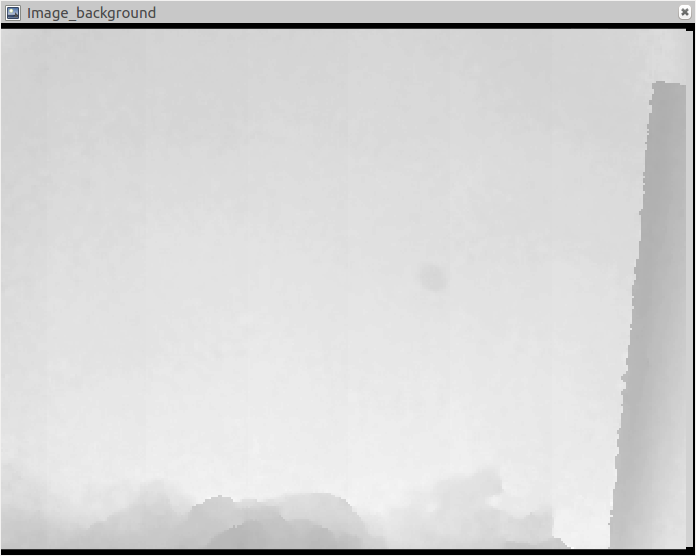
\includegraphics[width=0.5\linewidth]{background_02.png}
\caption{\label{fig:background2}The background stored at the beginning.}
\end{figure}

\begin{figure}
\centering
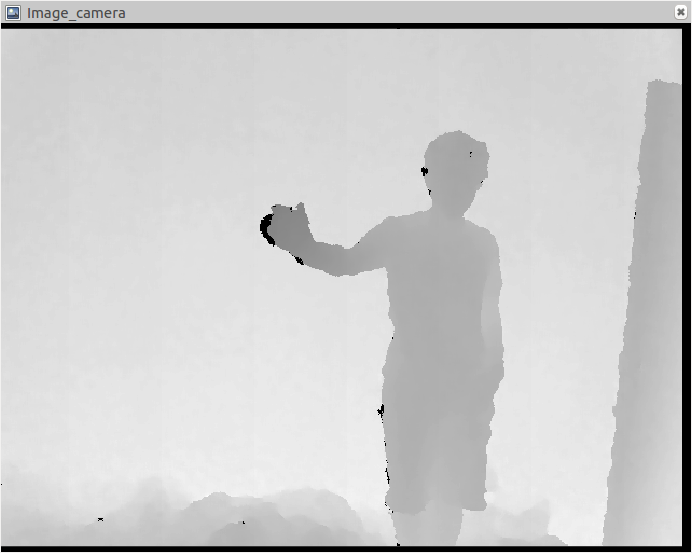
\includegraphics[width=0.5\linewidth]{camera_person_01.png}
\caption{\label{fig:cameraperson1}An image recorded while a person was in the field of view.}
\end{figure}

\begin{figure}
\centering
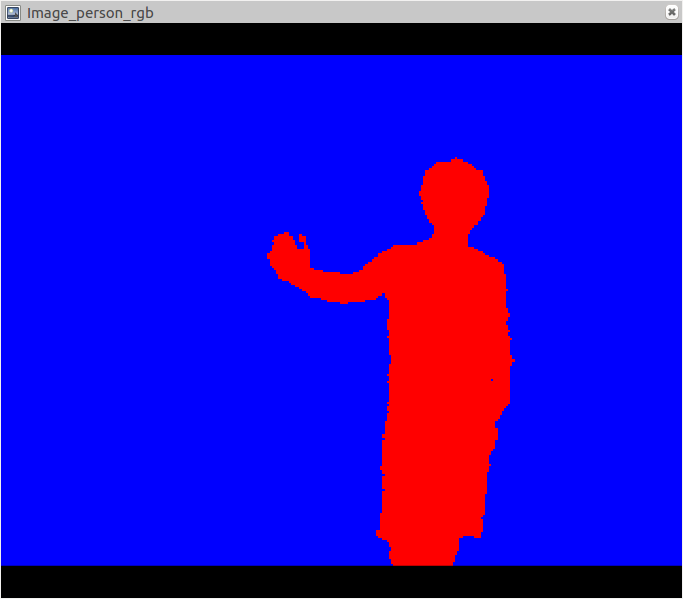
\includegraphics[width=0.5\linewidth]{clusters_person_01.png}
\caption{\label{fig:clustersperson1}The separation between static objects (in blue) and moving ones (in red).}
\end{figure}

To analyze the data provided by the sensor, we want first want to cut the image in two parts : the static objects (such as walls) and the dynamic, moving ones (cf Fig. \ref{fig:background2}, \ref{fig:cameraperson1}, \ref{fig:clustersperson1}). Existing studies already present person detection with RGB-D sensors, but with some limits, as sometimes persons won't be detected and on the other side static objects such as furniture will be identified as persons. This kind of problem could come from the fact that the camera could be moving.
In our case, we prefer static cameras along with high reliability detection, as we don't want to compromise security, as well as we don't want to stop the robot when it is too close to the table it is placed on. The static nature of the cameras allows to first store a reference background of the field of view when we start ; it requires the room to be empty of persons or robots. We then compute on each frame the differences between the frame and the background to get the dynamic objects. Afterwards, we want to separate the several objects we identified : it is known as clustering - each object being a cluster (cf Algo. \ref{algo:clustering}). The main challenge of this algorithm is to provide real-time reliable data ; the longest part is the $FuseTopAndLeftClusters()$ function, as the two clusters can be pretty big : a naive approach of re-computing the cluster for the whole image is not possible to stay above 1 frame per second.

\begin{algorithm}
\caption{\label{algo:clustering}3D Clustering : Compute the list of the clusters in the depth image}
\begin{algorithmic}
\REQUIRE $img[h][w]$ // the depth image
\STATE $cluster[h][w]$  // a tab to store the cluster of each pixel
\STATE 
\STATE // Start with the top-left corner
\IF{$isDynamic(img[0][0])$}
\STATE $cluster[0][0] \leftarrow NewCluster$
\ELSE
\STATE // This pixel belongs to the background
\STATE $cluster[0][0] \leftarrow Background$
\ENDIF
\STATE 
\STATE // Compute the left column
\FOR{$i:1 \rightarrow h-1$}
\IF{$isDynamic(img[i][0])$}
\IF{$diff(img[i-1][0], img[i][0]) < Threshold_{Depth}$}
\STATE // This pixel and the previous have similar depths : they are close and belong to the same object
\STATE $cluster[i][0] \leftarrow cluster[i-1][0]$
\ELSE
\STATE // This pixel and the previous one have different depths : they belong to different objects
\STATE $cluster[i][0] \leftarrow NewCluster$
\ENDIF
\ELSE
\STATE $cluster[i][0] \leftarrow Background$
\ENDIF
\ENDFOR
\STATE 
\STATE // Do the same for the upper line ($j:1 \rightarrow w-1$)
\STATE 
\STATE // Compute the rest of the image
\FOR{$i:1 \rightarrow h-1$}
\FOR{$j:1 \rightarrow w-1$}
\IF{$isDynamic(img[i][j])$}
\STATE $isNextToTopPixel \leftarrow diff(img[i-1][j], img[i][j]) < Threshold_{Depth}$
\STATE $isNextToLeftPixel \leftarrow diff(img[i][j-1], img[i][j]) < Threshold_{Depth}$
\IF{$isNextToTopPixel$ \AND $isNextToLeftPixel$ \AND Top and Left clusters are not already the same}
\STATE // This pixel connects two objects
\STATE $FuseTopAndLeftClusters()$
\ELSIF{$isNextToTopPixel$}
\STATE $cluster[i][0] \leftarrow cluster[i-1][0]$
\ELSIF{$isNextToLeftPixel$}
\STATE $cluster[0][j] \leftarrow cluster[0][j-1]$
\ELSE
\STATE $cluster[i][0] \leftarrow NewCluster$
\ENDIF
\ELSE
\STATE $cluster[i][j] \leftarrow Background$
\ENDIF
\ENDFOR
\ENDFOR
\end{algorithmic}
\end{algorithm}

\subsubsection{Noise minimization}

The cameras we are using are cheap, but it indeed has drawbacks, such as important noise (cf Fig. \ref{fig:camera1}) : these cameras use infra-red projection to get the depth data - cheaper than laser but less effective. We get important noise on these images (the black dots on Fig. \ref{fig:camera1}), often on smooth or glossy surfaces.
We need to get rid of those black dots, as they flicker on each frame, thus leading to identifying them as moving objects (cf Fig. \ref{fig:noise}). One known method of noise removal is to maintain a level on each pixel, increasing it when it is dynamic and decreasing it when static, to prevent single-frame noise. Our problem is that the noise we get flickers but stays at the same position, making this method irrelevant.
We therefore chose to simply remove the black dots - which give a depth value of 0 -, (as it represents around 95\% of the noise) from the background reference (by simply replacing them by the nearest non-zero value). We then consider all the zero depth values as static objects (cf Fig. \ref{fig:background1}).
However, there is still noise giving non-zero depth values, especially on far away surfaces. We chose to limit the zone of interest of the view to within 4 or 5 meters of the camera to avoid these problems.

\begin{figure*}[t!]
    \centering
    \begin{subfigure}[t]{0.5\textwidth}
        \centering
        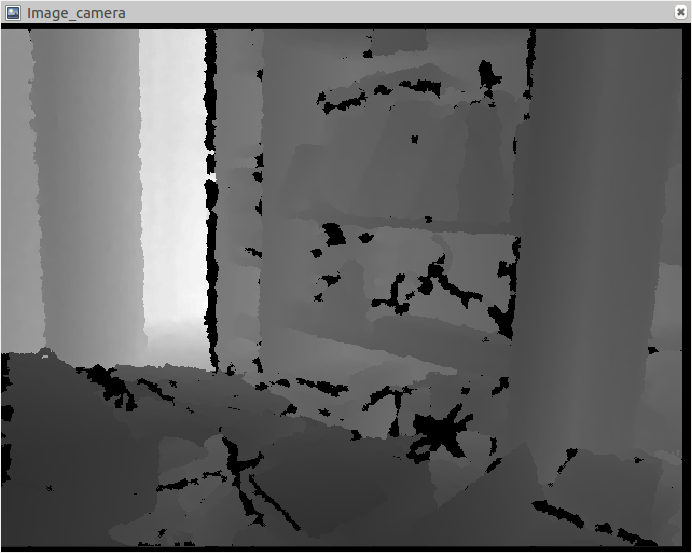
\includegraphics[height=0.8\textwidth]{camera_01.png}
        \caption{\label{fig:camera1}The depth image, as received by the camera : dark points are near the camera, bright ones are far.}
    \end{subfigure}
    ~ 
    \begin{subfigure}[t]{0.5\textwidth}
        \centering
        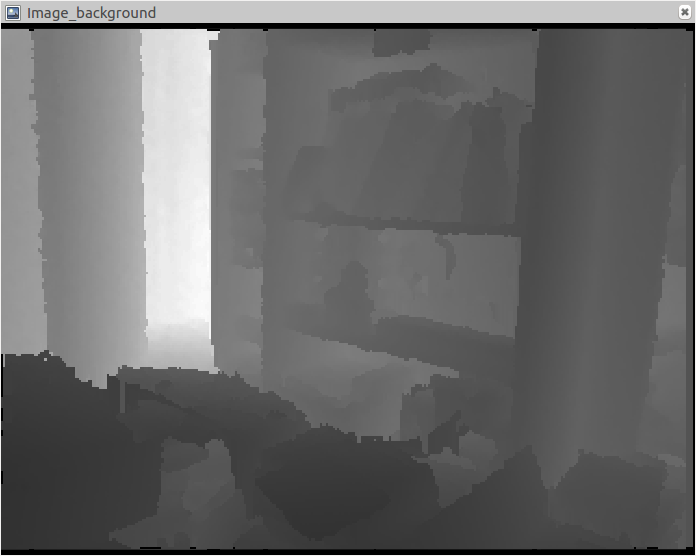
\includegraphics[height=0.8\textwidth]{background_01.png}
        \caption{\label{fig:background1}The same depth image after noise treatment.}
    \end{subfigure}
    \caption{Noise suppression}
\end{figure*}

\begin{figure}
\centering
\includegraphics[width=0.5\linewidth]{noise_02.png}
\caption{\label{fig:noise}Important noise interpreted as moving objects (in red and green).}
\end{figure}

\subsection{Identification}

Once we separated the several objects in the image, we need to identify persons and robots. AFZERJHGFSQDFKJDSF TODO

\section{The Distance-computing node}

The second node is in charge to compute the distance between each person and the robot. It receives data from the clustering node in the depth space, however distance computing is far easier in a cartesian space, thus we transpose coordinates in this space. The transposition of a point $P_d$ in the depth space to a point $P_c$ in the cartesian space is given by \[{P_c}_x = \frac{({P_d}_x-c_x){P_d}_z}{fs_x}, {P_c}_y = \frac{({P_d}_y-c_y){P_d}_z}{fs_y}, {P_c}_z = {P_d}_z \text{ \cite{Ref1}} \]
where $f,s_x,s_y,c_x,c_y$ are calibration data from the depth sensor (focal length, size of a pixel and coordinates of the focal axis in the image plane).

\begin{figure}
\centering
\includegraphics[width=0.6\textwidth]{depth_cartesian_spaces.png}
\caption{\label{fig:spaces}Representation of Cartesian space (a) and Depth space (b) \cite{Ref1}.}
\end{figure}

\section*{Acknowledgement}
This report is the result of a TER research internship at Université Grenoble Alpes, Grenoble, France.

%\subsection{How to add Tables}

%Use the table and tabular commands for basic tables --- see Table~\ref{tab:widgets}, for example. 

%\begin{table}
%\centering
%\begin{tabular}{l|r}
%Item & Quantity \\\hline
%Widgets & 42 \\
%Gadgets & 13
%\end{tabular}
%\caption{\label{tab:widgets}An example table.}
%\end{table}

%\subsection{How to write Mathematics}

%\LaTeX{} is great at typesetting mathematics. Let $X_1, X_2, \ldots, X_n$ be a sequence of independent and identically distributed random variables with $\text{E}[X_i] = \mu$ and $\text{Var}[X_i] = \sigma^2 < \infty$, and let
%\[S_n = \frac{X_1 + X_2 + \cdots + X_n}{n}
%      = \frac{1}{n}\sum_{i}^{n} X_i\]
%denote their mean. Then as $n$ approaches infinity, the random variables $\sqrt{n}(S_n - \mu)$ converge in distribution to a normal $\mathcal{N}(0, \sigma^2)$.


%\subsection{How to create Sections and Subsections}

%Use section and subsections to organize your document. Simply use the section and subsection buttons in the toolbar to create them, and we'll handle all the formatting and numbering automatically.

%\subsection{How to add Lists}

%You can make lists with automatic numbering \dots

%\begin{enumerate}
%\item Like this,
%\item and like this.
%\end{enumerate}
%\dots or bullet points \dots
%\begin{itemize}
%\item Like this,
%\item and like this.
%\end{itemize}

%\subsection{How to add Citations and a References List}

%You can upload a \verb|.bib| file containing your BibTeX entries, created with JabRef; or import your \href{https://www.overleaf.com/blog/184}{Mendeley}, CiteULike or Zotero library as a \verb|.bib| file. You can then cite entries from it, like this: \cite{greenwade93}. Just remember to specify a bibliography style, as well as the filename of the \verb|.bib|.

%You can find a \href{https://www.overleaf.com/help/97-how-to-include-a-bibliography-using-bibtex}{video tutorial here} to learn more about BibTeX.

%We hope you find Overleaf useful, and please let us know if you have any feedback using the help menu above --- or use the contact form at \url{https://www.overleaf.com/contact}!

%\bibliographystyle{alpha}
%\bibliography{sample}
\begin{thebibliography}{}

\bibitem{Ref1}
F. Flacco and A. De Luca, Real-time computation of distance to dynamic obstacles with multiple depth sensors, IEEE Robotics and automation Letters (2016).
http://comanoid.cnrs.fr/publications\_files/2017/IEEE\_Robotics\_and\_Automation\_Letters/RAL2016\_MultiDepth\_preprint.pdf

\bibitem{Ref2}
F. Flacco, T. Kröger, A. De Luca and O. Khatib, A depth space approach for evaluating distance to objects, J. of Intelligent and Robotic Systems, vol. 80 (suppl. 1), pp 7-22 (2015).
http://www.dis.uniroma1.it/\textasciitilde labrob/pub/papers/JINT14\_DepthSpace\_final.pdf

\bibitem{Ref3}
F. Flacco, T. Kröger, A. De Luca and O. Khatib, A depth space approach to human-robot collision avoidance, Proc. IEEE Int. Conf. on Robotics and Automation, pp. 2353-2359 (2013).
https://cs.stanford.edu/group/manips/publications/pdfs/Flacco\_2012\_ICRA.pdf

%\bibitem{Ref4}
%L.  Balan  and  G.  Bone,  Real-time  3D  collision  avoidance  method for safe human and robot coexistence, Proc. IEEE Int. Conf. on Intelligent  Robots  and  Systems, pp. 276–282 (2006).

\bibitem{Ref5}
P. Jia, S. Ioan, C. Sachin and M. Dinesh, Real-time collision detection and  distance computation  on  point  cloud  sensor data, Proc.  IEEE Int. Conf. on Robotics and Automation, pp. 3593–3599 (2013).
http://ioan.sucan.ro/files/pubs/realtime\_cd\_sensor\_data\_icra\_2013.pdf

\bibitem{Ref6}
C. Morato, K.N. Kaipa, B. Zhao and S.K. Gupta, Toward Safe Human Robot Collaboration by using Multiple Kinects based Real-time Human Tracking, Journal of Computing and Information Science in Engineering (2014).
http://www.enme.umd.edu/\textasciitilde skgupta/Publication/JCISE2013\_Morato\_draft.pdf

\bibitem{Ref7}
N. Najmaei and M. Kermani, Prediction-based reactive control strategy for human-robot interactions, IEEE Int. Conf. on Robotics and Automation (ICRA), pp. 3434–3439 (2010).
https://pdfs.semanticscholar.org/19b6/b377548396e47c90d5c5ea6630a265016a22.pdf

\bibitem{Refopenni}
http://wiki.ros.org/openni\_camera

\end{thebibliography}

\end{document}
